\documentclass{standalone}

% Preamble
\begin{document}

  \subsection{Numerical experiment}

In this experiment, we solve the particular polynomial system $f = [\\ 
\input{txt/P.txt}$
]\\
The size of the Bezout matrix $B(1)$ is $\input{txt/Dx.txt}$; this is the maximum number of solutions that a system of degree \input{txt/deg.txt} can have. To initiate the reduction process, the rank of $B(1)$ is needed; as the matrix has integer coefficients, we use the Sage function matrix.kernel() to calculate its rank. This is the only computation that we do in exact arithmetic; all the subsequent computations are done in floating-point arithmetic.
After the reduction process has been completed, we find that the dimension of the quotient $A$ is $\input{txt/bezout_dim.txt}$.
Since the computations have been done numerically, the Bezout matrices and the companion matrices are numerical matrices and the eigenvalues of the companion matrices $X_j = B(x_j)B(1)^{-1}$ are numerical approximations of the roots of the polynomial system $f$.

\subsubsection{Quality of the results}
To check the quality of the numerical roots $\alpha$, we compute the errors $f(\alpha)$.
These errors are shown in 

\iffalse
an histogram (Figure \ref{fig:roots}).
\begin{figure}[p]
    \caption{Histogram of errors}
  \label{fig:roots}
  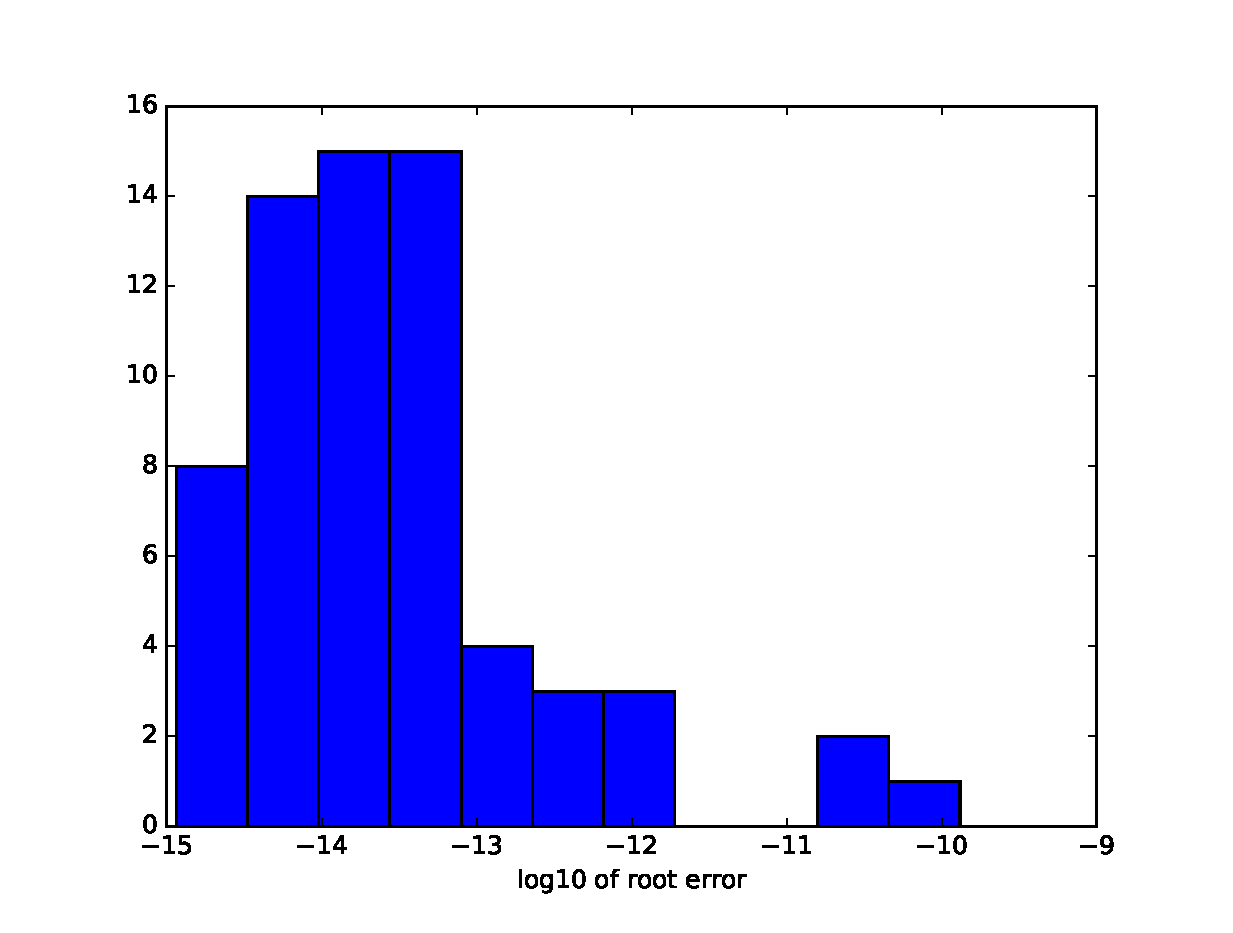
\includegraphics[scale=0.5]{txt/histo_roots.eps}
\end{figure}
\fi

a table

\subsubsection{Timings}
Table \ref{tab:timings} shows the timings of the Bezout computations as compared to the timings of the  Groebner computations.
\begin{table}[p]
    \caption{timings}
\label{tab:timings}
\begin{tabular}{llllr}
 Méthode & Computation & Software & Arithmetic & Timing \\ \hline
   \multirow{4}{*}{Bezout} & Bezout matrices & NumPy & floating point & $\input{txt/construction_B_time.txt}$ s \\
   & rank of $B(1)$ via rref()  & Sage & integer & $\input{txt/b0_rref_time.txt}$ s \\
   & matrices reduction & Numpy & floating point & $\input{txt/reductions_time.txt}$ s \\
   & eigenvalues & SciPy & floating point & $\input{txt/compute_roots_time.txt}$ s \\ 
   \hline
   \hline
   Groebner & Groebner basis computation & Sage & integer & $\input{txt/groebner_time.txt}$ s
\end{tabular}
\end{table}



\end{document}
